\documentclass[10pt,landscape]{article}
\usepackage{multicol}
\usepackage{calc}
\usepackage{setspace}
\usepackage{ifthen}
\usepackage[landscape]{geometry}
\usepackage{graphicx}

% To make this come out properly in landscape mode, do one of the following
% 1.
%  pdflatex latexsheet.tex
%
% 2.
%  latex latexsheet.tex
%  dvips -P pdf  -t landscape latexsheet.dvi
%  ps2pdf latexsheet.ps


% If you're reading this, be prepared for confusion.  Making this was
% a learning experience for me, and it shows.  Much of the placement
% was hacked in; if you make it better, let me know...


% 2008-04
% Changed page margin code to use the geometry package. Also added code for
% conditional page margins, depending on paper size. Thanks to Uwe Ziegenhagen
% for the suggestions.

% 2006-08
% Made changes based on suggestions from Gene Cooperman. <gene at ccs.neu.edu>


% To Do:
% \listoffigures \listoftables
% \setcounter{secnumdepth}{0}


% This sets page margins to .5 inch if using letter paper, and to 1cm
% if using A4 paper. (This probably isn't strictly necessary.)
% If using another size paper, use default 1cm margins.
 \geometry{top=.2in,left=.2in,right=.2in,bottom=.2in} 


% Turn off header and footer
\pagestyle{empty}
 

% Redefine section commands to use less space
\makeatletter
\renewcommand{\section}{\@startsection{section}{1}{0mm}%
                                {-1ex plus -.5ex minus -.2ex}%
                                {0.5ex plus .2ex}%x
                                {\normalfont\large\bfseries}}
\renewcommand{\subsection}{\@startsection{subsection}{2}{0mm}%
                                {-1explus -.5ex minus -.2ex}%
                                {0.5ex plus .2ex}%
                                {\normalfont\normalsize\bfseries}}
\renewcommand{\subsubsection}{\@startsection{subsubsection}{3}{0mm}%
                                {-1ex plus -.5ex minus -.2ex}%
                                {1ex plus .2ex}%
                                {\normalfont\small\bfseries}}
\makeatother

% Define BibTeX command
\def\BibTeX{{\rm B\kern-.05em{\sc i\kern-.025em b}\kern-.08em
    T\kern-.1667em\lower.7ex\hbox{E}\kern-.125emX}}

% Don't print section numbers
\setcounter{secnumdepth}{0}


\setlength{\parindent}{0pt}
\setlength{\parskip}{0pt plus 0.5ex}


% -----------------------------------------------------------------------


\begin{document}

\raggedright
\footnotesize
\begin{multicols}{3}


% multicol parameters
% These lengths are set only within the two main columns
%\setlength{\columnseprule}{0.25pt}
\setlength{\premulticols}{1pt}
\setlength{\postmulticols}{1pt}
\setlength{\multicolsep}{1pt}
\setlength{\columnsep}{2pt}

\begin{center}
     \Large{\textbf{CS 211 Cheat Sheet}} \\
\end{center}

\section{Base Arithmetic and Conversions}


To convert {\bf decimal to binary}, divide by 2 and if remainder is even the binary remainder is 0,
else 1. Take the first digit and work up to the last.

{\bf Hex arithmetic} is done by adding normally and converting to base $16$, i.e. $17 + A7$
becomes $7 + 7 = 14 = E$, and then $1 + A = 11 = B$ so we get $BE$

{\bf Hex multiplication} is the same as base-10, except we end up subtracting by
16 when we get the sum. $21 \times 2 = (2 \times 1) + (20 \times 2) = 42$


\begin{center}
\begin{tabular}{|ccc|ccc|}
    \hline
    Hex & Binary & Decimal & Hex & Binary & Decimal \\ \hline
    0   & 0000   & 0       & 8   & 1000   & 8       \\ \hline
    1   & 0001   & 1       & 9   & 1001   & 9       \\ \hline
    2   & 0010   & 2       & A   & 1010   & 10      \\ \hline
    3   & 0011   & 3       & B   & 1011   & 11      \\ \hline
    4   & 0100   & 4       & C   & 1100   & 12      \\ \hline
    5   & 0101   & 5       & D   & 1101   & 13      \\ \hline
    6   & 0110   & 6       & E   & 1110   & 14      \\ \hline
    7   & 0111   & 7       & F   & 1111   & 15      \\ \hline
\end{tabular}
\end{center}

\section{De Morgan's Law}

% Prove De Morgan’s Law
% Truth tables

\begin{center}
\begin{tabular}{|l|l|l|l|l|l|l|l|l|l|}
    \hline
    $\lnot$ & $(A$ & $\land$ & $B)$ & $\equiv$ & $(\lnot$ & $A)$ & $\lor$ & $(\lnot$ & $B)$ \\ \hline
    F       & T    & T       & T    & T        & F        & T    & F      & F        & T    \\
    T       & T    & F       & F    & T        & F        & T    & T      & T        & F    \\
    T       & F    & F       & T    & T        & T        & F    & T      & F        & T    \\
    T       & F    & F       & F    & T        & T        & F    & T      & T        & F    \\ \hline
\end{tabular}
\end{center}

\section{Pipelining}

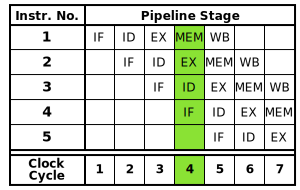
\includegraphics[scale=.9]{pip}

The process of taking multiple instances of one process and streamlining it.  By pipelining, you shorten the total amount of time for things to be 
done, but often have to make a certain step of the process take longer.  Without pipelining, instance one would go A to B to C and instance two 
would start when it completes. With pipelining, instance one finishes A, stores that value in a register, begins instance B and as it begins B 
instance 2 begins A, etc until it is completed.

{\bf General Pipelining} is the idea that there is no reason to ever have idle hardware in a computer. INSTRUCTION 

{\bf Pipelining} is when each instruction step is split up and consecutive instructions are executed at the same time. IN 

{\bf Order}: Instruction Fetch, instruction Decode, Execute, Memory access, register write back.

{\bf Data dependency}: the output of one instruction is an input to another.

{\bf Control dependency}: some instruction determines the location of the instruction to execute call, return jump

{\bf Dealing by Stalling}: prevent the execution of an instruction until the outputs of the previous instructions(use no-ops to stall)

{\bf Dealing by Forwarding}: make output values available to earlier instructions. Just keep executing instructions, look at pending values instead of 
current value and get it.

\textbf{Structural hazards} commonly occurs when two activites require the same resource. \textbf{Solution:} We stall the pipeline when if it occurs.
A \textbf{Control hazard} are a type of hazard that occur from an uncertain execution path,
either a \textit{possible branch} or a \textit{branch not taken}. \textbf{Solution:} A stall, or by delaying the branch.
\textbf{Data hazards} occur when the pipeline changes the order of read/write access, 
or when some instruction is \textit{dependant} on the outcome of a previous instruction 
not yet completed. \textbf{Solution:} Internal forwarding.

\section{Random Access Memory}

{\bf RAM} is the primary means for a computer to run programs in real time. RAM is designed to be fast and dense, but most RAM is also volatile, meaning that information is lost quickly when there is no power provided to the chip.

\subsection{Static}
{\bf SRAM} is more expensive because it takes several transistors and capacitors per each bit of memory, making it naturally less dense. The advantages for SRAM are as follows: It is faster, and it has constant-time direct address access. It also, depending on the implementation, can be much less power dependent.

\subsection{Dynamic}
{\bf DRAM} is the simplest form of storage available, each bit is just one capacitor that either has a charge or does not have a charge. This makes DRAM extremely memory dense, and very very very cheap. The problem is that, because capacitors lose charge quickly, each address has to be ``refreshed'' (re-charged) periodically to avoid loss of information. This makes it slow and power inefficient.

\subsection{Why is DRAM so slow?}
{\bf DRAM is slow}, relative to SRAM, because so much effort is expended to make sure that the information you are accessing is the information that you want and not some corruption due to loss of charge.

Furthermore, {\bf DRAM} is arranged as a 2D array, and this is why it is slower to access. We must go
row then column, or column then row. These are known as {\bf Row Access
Strobe} and {\bf Column Access Strobe requests}.

DRAM requires data to be refreshed from time to time in order to keep the data
SRAM does not need to be refreshed, since the transistors inside continue to hold the data as long as power supply is on. DRAM contains more circuitry, and requires more timing for the refresh, creating complications that make it slower than SRAM (higher power requirement is such a complication)
SRAM is simpler compared to DRAM, but need more transistors than DRAM. DRAM generally need a single transistor for each bit of data, but SRAM need 6 (this is why DRAM is cheaper and larger)

\section{Caches}

{\bf Block}: a fixed chunk of data that moves back and forth between cache and main memory. 

{\bf Set}: collection of lines. 

{\bf Working Set}: set of blocks we are using now, changes through execution. 

{\bf Capacity}:  total number of bytes that it can hold. Obtained by the number of blocks multiplied by the size, where the blocks is the number of sets multiplied by the number of lines per set. 

{\bf Cold Miss}: occurs when memory location is accessed for the first time. 

{\bf Conflict Miss}:  occurs when the level cache is large enough, but multiple data items all map to the same k block. 

{\bf Cache Hit}: when we look for something and it is there. 


{\bf Fully associative}: allowed to choose any entry

{\bf Set associative}:  more than one line per set, powers of 2. All
must have same amount.

{\bf Direct-mapped cached}: simplest kind, one line per set.

\section{Endianness}

Two forms of Endian-ness (big endian, little endian), which refer to the ordering of bytes stored in memory, determined by significance of byte. 
Little endian store least significant byte first, at lowest byte address (most machines) and big endian store most significant byte first at lowest 
byte address.

Two kinds, Big endian and Little endian. Big endian is MSB first,
decreasing numeric significance as byte address increases. Little
endian is LSB first, with an increasing numeric significance as the
address increases (Intel uses this). For example, storing \texttt{0A0B0C0D}:
Big Endian - \texttt{0A 0B 0C 0D}; Little Endian \texttt{0D 0C 0B 0A}

\section{LRU and LFU algorithms}

{\bf Least Recently Used} (LRU): discards the least recently used items first. This algorithm requires keeping track of what was used when, which is expensive if one wants to make sure the algorithm always discards the least recently used item.

Least recently used works by using system clock to determine when cache was used recently. Caches that were used a long time ago are evicted 
first

We always increment global counter by one for any block. If the block we are looking for is already in the cache, we set the counter for 
the block to the global access counter. If it is not in the cache, we get the block, put it in the cache, and set its count equal to the global 
counter. You put an ``event time'' on the block.  Event timer is another step forward in time—keep accessing the same block, they they 
move forward. The block we used furthest in past gets evicted.

{\bf Least Frequently Used} (LFU): LFU counts how often an item is needed. Those that are used least often are discarded first.

The simplest method to employing an LFU algorithm is to assign a counter to every block that is loaded into the cache. Each time a reference is made to that block the counter is increased by one. When the cache reaches capacity and has a new block waiting to be inserted the system will search for the block with the lowest counter and remove it from the cache.

Least frequently used works by using hardware flags to determine how many times something is used. Least frequently used cache is evicted 
(duh). There's some problems with this since something can be used a lot at the beginning and then not be used at all afterward.

Every block as an integer usage counter, initialized to one. Every time a block in cache is accessed, increment it. When it comes time to 
evict, select the block with the lowest counter value.  Read in a new block and the counter is set to one (because of locality, we increment 
it).

\emph{Limitations}: if we use a block a lot and stop using it, it won't be evicted even though it is not being currently used a lot.

$$T = m*T_m + T_h + E$$

$T$ = average memory reference time

$m$ = miss ratio = 1 - (hit ratio)

$T_m$ = time to make a main memory access when there is a miss (or, with multi-level cache, average memory reference time for the next-lower cache)

$T_h$ = the latency: the time to reference the cache when there is a hit

$E$ = various secondary effects, such as queuing effects in multiprocessor systems

\section{x86 Instructions}

\begin{center}
\begin{tabular}{|p{1.1cm}|p{6cm}|}
    \hline
\texttt{mov} & copies data from the second operand to the first. Can not do memory to memory.\\\hline
\texttt{lea} & places address of second operand into the register of the first.\\\hline
\texttt{add} & adds two operands together, stored in the first operand.\\\hline
\texttt{sub} & subtracts two operands together, stored in the first operand.\\\hline
\texttt{imul} & multiplies two operands together and stores it in the first operand.\\\hline
\texttt{and, or, xor} & applies the bitwise operator on two operands, stored in the first operand.\\\hline
\texttt{jumps} & jumps to a label depending on location.\\\hline
\texttt{cmp} & nondestructive subtraction.\\\hline
\end{tabular}
\end{center}

\section{Call Stack}

Stack {\bf grows downards} (high to low addresses). The top is the \%esp
register. The frame pointer, or \%ebp serves a fixed location, such as the
return address. The portion allocated for a single procedure is called a
stack frame.

\texttt{push}: set the stack pointer to
\texttt{\%esp = \%esp − (4 times the number of registers)}

\texttt{pop}: copy the data from the stack to the registers, then
\texttt{\%esp = \%esp + 4( times the number of registers)}

Having a frame pointer is convenient when a function is likely to move
the stack pointer several times throughout the course of running the
function.

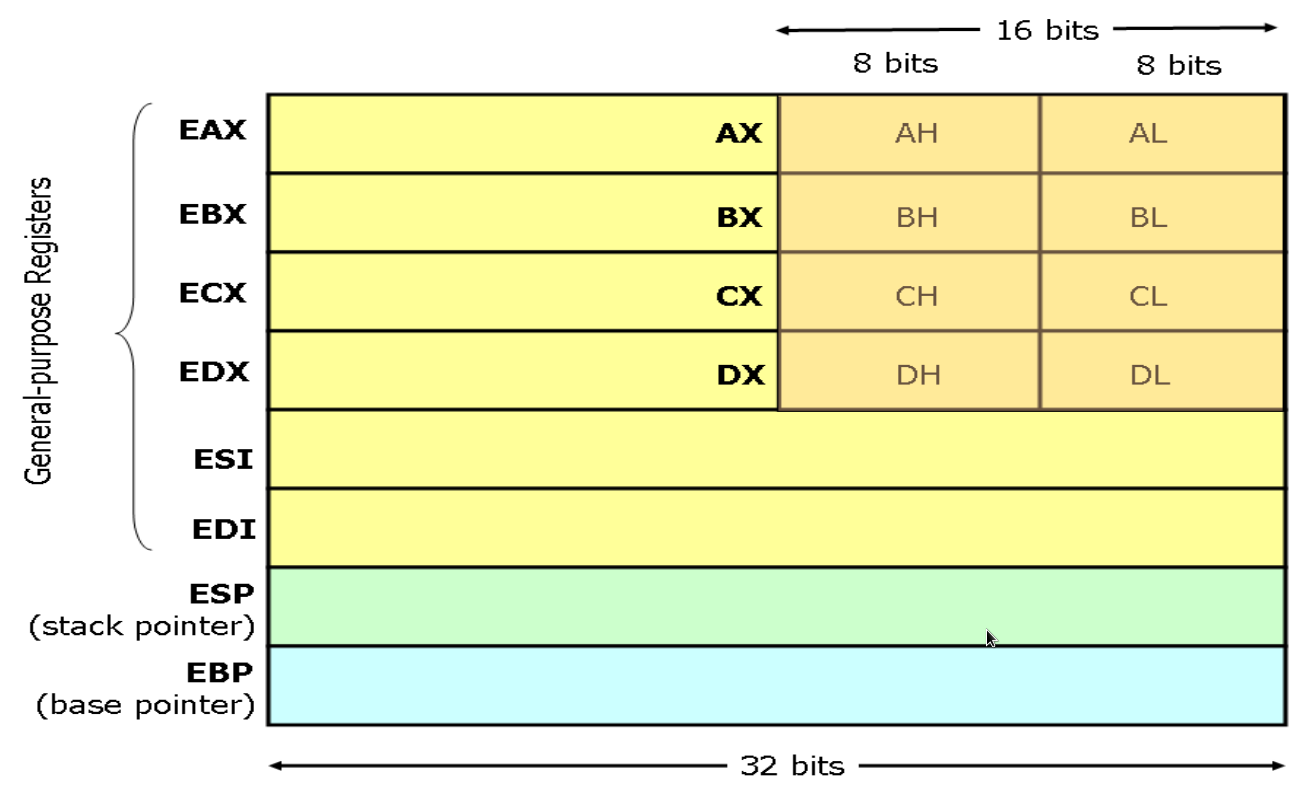
\includegraphics[scale=.175]{reg}

\section{Karnaugh Maps}

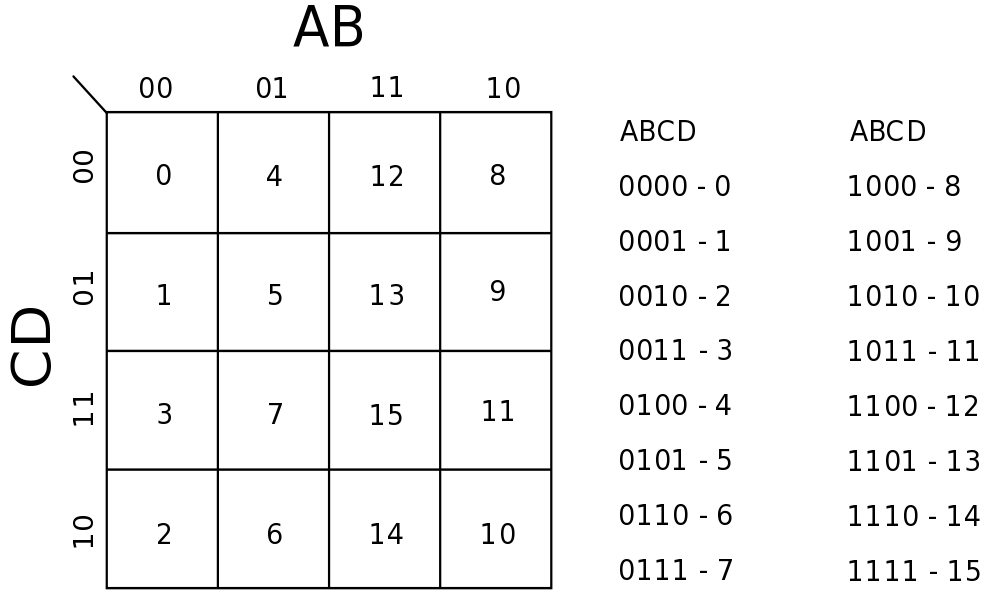
\includegraphics[scale=.3]{kar}

Solving a Karnaugh Map: (1) Group rectangles that are touching;
(2) Each rectangle is an or statement;
(3) Remember that they can “wrap” from side to side.

\section{Drawing a Circuit}

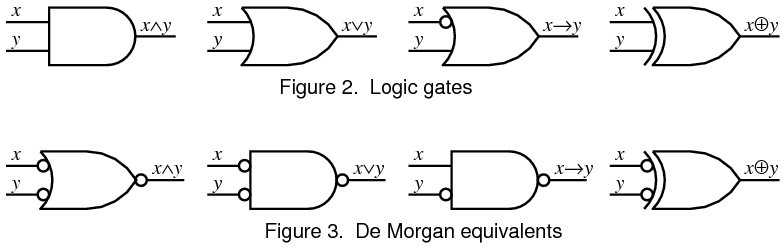
\includegraphics[scale=.3]{log}

% Draw a circuit

\section{Locality}

{\bf Good locality} allows a program to run faster than one with poor locality.
Stride-k is sequential visiting pattern, for example visiting every space
in an array is of stride 1, with every k − t h element being stride k.

{\bf Temporal Locality} occurs when things occur over a short
period of time next to each other.

memory that is referenced once is likely to be referenced again (the more you use one thing, the better). As an example, 
using the same variable in a summation for loop instead of using multiple variables. 

{\bf Spatial Locality} occurs when things are close together in
memory/space. As stride increases, the spatial locality
decreases. (keep memory that you use a lot close by to each other.)

For example, the elements in an array, \texttt{arr} will have spatial locality.
Accessing \texttt{i} and \texttt{arr[i]} happen after each other, so they have
temporal locality.

\section{Writing Policies}

{\bf Write-through}: Every time you write something to a cached block, you write it through to whatever is below this block. If you write to L1, then you also  write to L2. \emph{Advantages}: easy with software and hardware, always consistent, good if reads is greater than writes. \emph{Disadvantages}: if writes is greater than reads, lose a significant amount of speed

{\bf Write-back}: Only when a page is evicted do you write it to the lower level. Usually the larger a block is, the more likely they are to be write-back. \emph{Advantages}: faster, smaller number of downward block transfers; \emph{Disadvantages}: harder to implement, greater possibility of data inconsistency

{\bf Writing to blocks not in cache}: 

\emph{Write-allocate}: Puts the block in the cache, so subsequent writes also go to the cache. Advantages: takes advantage of spacial locality. Disadvantages: every miss requires a block transfer upwards, causing a block eviction

\emph{No-Write-Allocate}: Does not take advantage of spacial locality (write-through is typically no-write-allocate)

\section{Addressing Modes}

\begin{tabular}{|p{2.55cm}|p{3.65cm}|}
\hline
{\bf Instruction} (mov) & {\bf Result} \\\hline
eax, ebx & ebx = eax \\
(eax), ebx & ebx = mem[eax] \\
4(eax), ebx & ebx = mem[eax+4] \\
(eax, ecx), ebx & ebx = mem[eax+ecx] \\
4(eax, ecx), ebx & ebx = mem[eax+ecx+4] \\
(eax, ecx, 2), ebx & ebx = mem[eax+ecx*2] \\
4(eax, ecx, 2), ebx & ebx = mem[eax+ ecx*2 +4] \\\hline
\end{tabular}

\section{Two's Complement}

Gives us the ability to represent negative values. In binary, negative
numbers start with a 1 and positive numbers start with a 0. For
example, we will use 00002710. In order to find the two’s complement
form of a number, we do two steps: (1) Flip - we flip the bits to become FFFFD8EF.
(2) Add One - we add one to the number, becoming FFFFD8F0.


\section{Shifting}
There are two types:
\textbf{Left Shift} moves bytes to the left. Same as multiplying $2^n$.
\textbf{Right Shift} moves bytes to the left. Same as dividing $2^n$.

Each has two forms:
\textbf{Arithmetic} preserves sign.
\textbf{Logical} means our new high bits are zero, including sign.

\section{Floating points}

First bit is the sign bit which determines if the number is positive or
negative. The next are the exponent. The rest are fraction for the
number.

\section{Assembly to C}
Depending on syntax, \texttt{addl r1,r2} becomes \texttt{r2 = r1+r2}. Jumps and conditions allow us to create loops.
An auto array will be made by \texttt{movl \%edx, -48(\%rbp,\%rax,4)} and scaled by 4 because it is an int array.
Accessing a struct array is \texttt{movl \%edx, a+8(,\%rax,4)} where \texttt{a} is the name of the struct.
Row major access of a matrix is \texttt{movl \%ecx, array(,\%rax,4)}.

\end{multicols}
\end{document}
